%!TEX root = ../main.tex 

\section{Comment protéger une alimentation?}

\subsection{Protection antistatique}

\begin{frame}{Décharge Électrostatique (ESD)}
    \begin{columns}
        \begin{column}{0.66\textwidth}
            \begin{itemize}
                \item Norme IEC-61000-4-2
                \begin{itemize}
                    \item Types de décharges
                    \item Méthodologies de tests \& certification
                    \item 4 catégories de produits
                    \item Jusqu'à $\SI{\pm 8}{\kilo\volt}$ / $\SI{\pm 15}{\kilo\volt}$
                \end{itemize}
                \item Deux types de chocs statiques
                \begin{itemize}
                    \item \textbf{Contact Discharge} - Toucher directement chaque pin avec un ESD gun
                    \item \textbf{Air Discharge} - ESD gun proche du DUT jusqu'à décharge
                \end{itemize}
            \end{itemize}
        \end{column}

        \begin{column}{0.33\textwidth}
            \begin{figure}
                \centering
                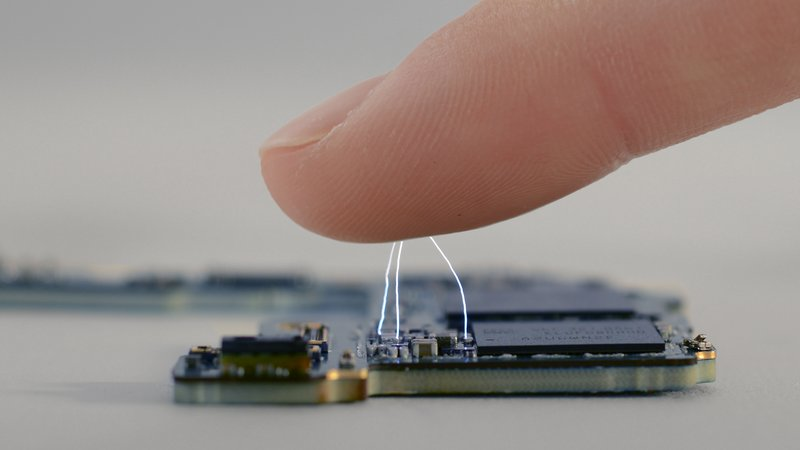
\includegraphics[width=\textwidth]{pictures/ESD-discharge-finger.png}
            \end{figure}
            \begin{figure}
                \centering
                
\includegraphics[width=0.5\textwidth]{pictures/ESD-logo.png}
            \end{figure}
        \end{column}
    \end{columns}
\end{frame}

\begin{frame}{Décharge Électrostatique - Waveform}
    \begin{columns}
        \begin{column}{0.5\textwidth}
        \end{column}
        \begin{column}{0.5\textwidth}
            \begin{itemize}
                \item Pic de courant initial
                \begin{itemize}
                    \item Rise time $\lesssim \SI{1}{\nano\second}$
                \end{itemize}
                \item $2^e$ pic
                \item Chute graduelle
            \end{itemize}
        \end{column}
    \end{columns}

    \vspace{-66pt}

    \begin{figure}
        \centering
        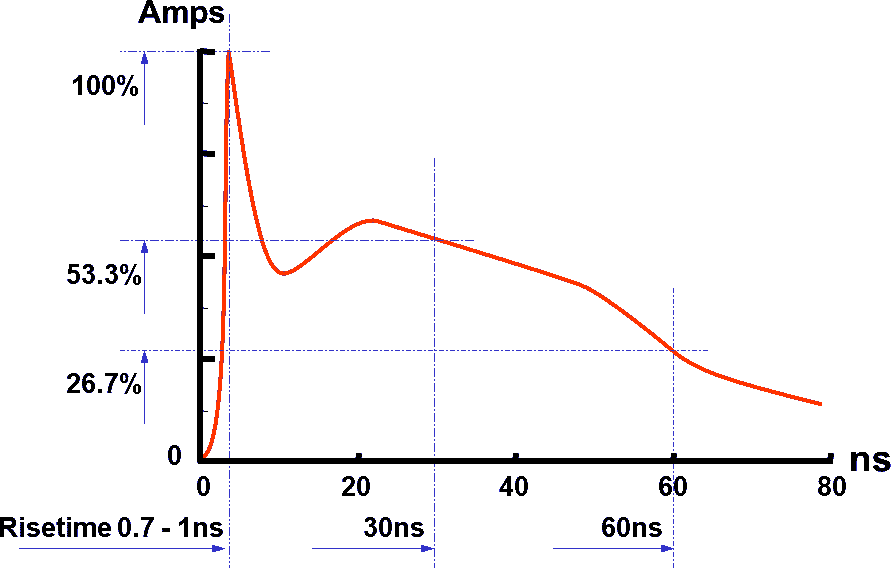
\includegraphics[width=\textwidth]{pictures/ESD-discharge-waveform.png}
    \end{figure}
\end{frame}

\begin{frame}{Circuit protégé antistatiquement - Zener}
    \begin{center}
    \vspace{-24pt}
    \resizebox{\textwidth}{!}{
    \begin{circuitikz}[american voltages]
        \draw [thick]
        (0,-3) to [short, *-] (10,-3)
        to [european resistor, l_=${LOAD}$] (10,1)
        (0,-3) to [open, v<=$V$] (0,1)
        to [short] (10,1)
        ;

        \draw [thick]
        (3, -3) to [empty ZZener diode, color=red] (3, 1);

        % Current spike as a waveform
        \draw[thick, ->] (-0.1, 2) -- (0,3) % Rising edge
        -- (0,3) -- (0.1,1.8) % First sharp drop
        -- (0.2,2.5) -- (0.3,1.9) % Second spike
        -- (0.4,2.3) -- (0.5,2.0) % Smaller oscillation
        -- (0.6,2.15) -- (0.7,2.05) % Final damping
        -- (1,2.1); % Settling

        \node[right] at (1,2.1) {$i_{\text{ESD}}(t) \rightarrow \SI{8}{\kilo\volt}$};
    \end{circuitikz}
    }
    \end{center}
\end{frame}

\begin{frame}{Diode Normale - IV Curve}
    \begin{figure}
        \centering
        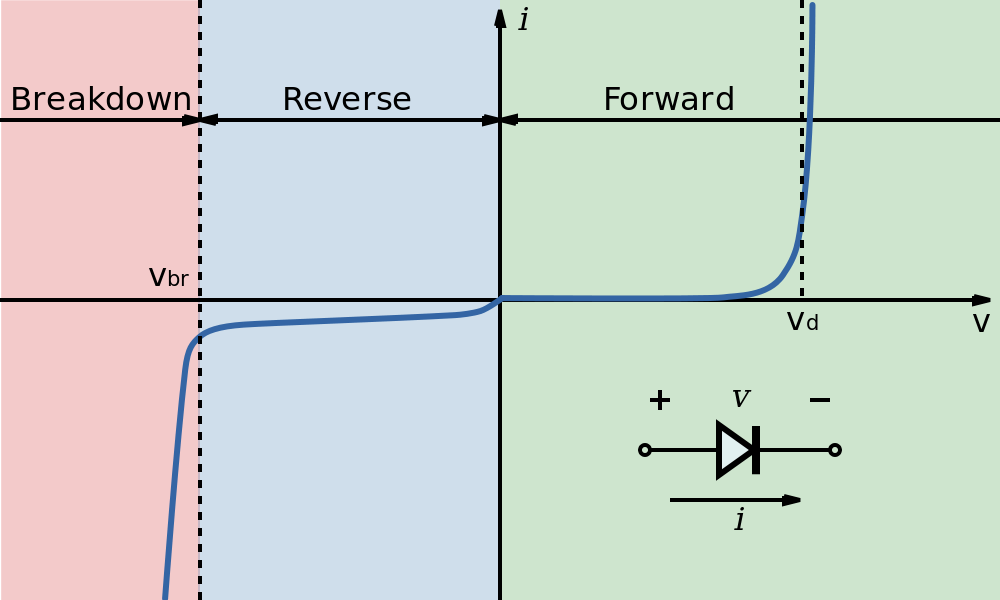
\includegraphics[width=\textwidth]{pictures/diode-iv-curve.png}
    \end{figure}
\end{frame}

\begin{frame}{Diode Zener}
    \begin{columns}
        \begin{column}{0.4\textwidth}
            \begin{itemize}
                \item \textbf{Faite pour être mise à l'envers!}
                \bigskip
                \item $V_Z$ contrôlé
                \item Beaucoup de courant en avalanche
                \item N'endommage pas la diode
                \bigskip
                \item Utilisé dans des références de tension
                \item Utilise comme protection antistatique
            \end{itemize}
        \end{column}
        \begin{column}{0.6\textwidth}
            \begin{figure}
                \centering
                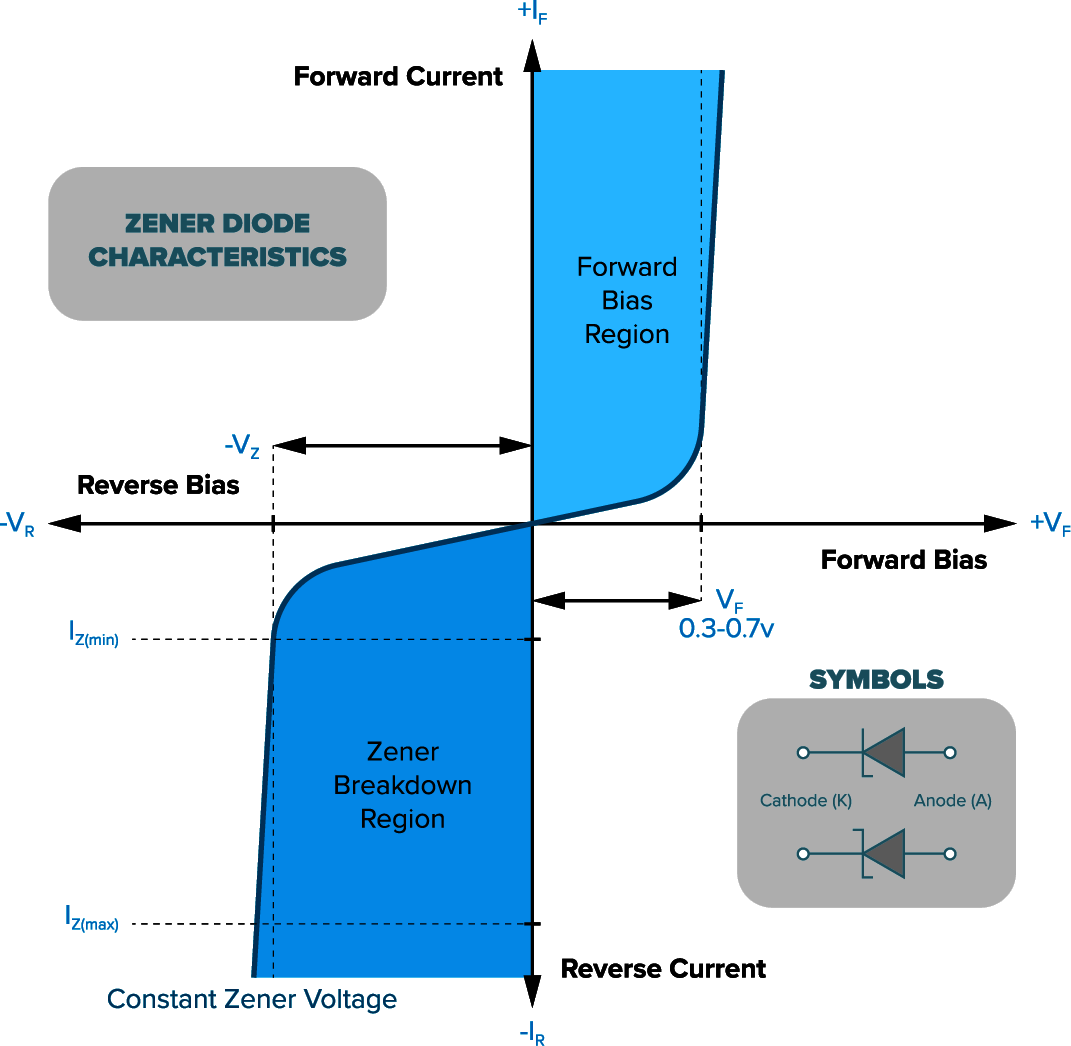
\includegraphics[width=\textwidth]{pictures/diode-zener-iv-curve.png}
            \end{figure}
        \end{column}
    \end{columns}
\end{frame}

\begin{frame}{Circuit protégé antistatiquement}
    \begin{center}
    \vspace{-24pt}
    \resizebox{\textwidth}{!}{
    \begin{circuitikz}[american voltages]
        \draw [thick]
        (0,-3) to [short, *-] (10,-3)
        to [european resistor, l_=${LOAD}$] (10,1)
        (0,-3) to [open, v<=$V$] (0,1)
        to [short] (10,1)
        ;

        \draw [thick]
        (3, -3) to [full ZZener diode, a=$\SI{15}{\volt}$] (3, 1);

        \draw[->, thick, red] 
        (1, 0.75) to[out=0, in=90] (2.75, -0.5);

        % Current spike as a waveform
        \draw[thick, ->]
           (-0.1, 2) -- (0,3)       % Rising edge
        -- (0,3) -- (0.1,1.8)       % First sharp drop
        -- (0.2,2.5) -- (0.3,1.9)   % Second spike
        -- (0.4,2.3) -- (0.5,2.0)   % Smaller oscillation
        -- (0.6,2.15) -- (0.7,2.05) % Final damping
        -- (1,2.1);                 % Settling

        \node[right] at (1,2.1) {$i_{\text{ESD}}(t) \rightarrow \SI{8}{\kilo\volt}$};
    \end{circuitikz}
    }
    \end{center}
\end{frame}


\begin{frame}{Protection avec une diode Zener}
    \begin{itemize}
        \item Clamp le pulse à $V_Z$
        \item Protège les dispositifs par apprès
        \bigskip
        \item Pas l'option la plus rapide
        \item Ne protège pas contre un pulse négatif 
    \end{itemize}

    \begin{figure}
        \centering
        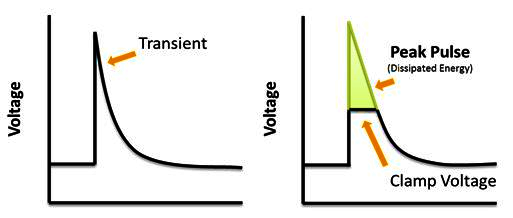
\includegraphics[width=\textwidth]{pictures/clamping-esd-pulse.png}
    \end{figure}
\end{frame}


\begin{frame}{Circuit protégé antistatiquement - TVS}
    \begin{center}
    Circuitikz version here is \pgfcircversion{} released on \pgfcircversiondate{}.
    \vspace{-24pt}
    \resizebox{\textwidth}{!}{
    \begin{circuitikz}[american voltages]
        \draw [thick]
        (0,-3) to [short, *-] (10,-3)
        to [european resistor, l_=${LOAD}$] (10,1)
        (0,-3) to [open, v<=$V$] (0,1)
        to [short] (10,1)
        ;

        \draw [thick]
        (3, -3) to [empty ZZener diode, color=red] (3, 1);

        % Current spike as a waveform
        \draw[thick, ->] (-0.1, 2) -- (0,3) % Rising edge
        -- (0,3) -- (0.1,1.8) % First sharp drop
        -- (0.2,2.5) -- (0.3,1.9) % Second spike
        -- (0.4,2.3) -- (0.5,2.0) % Smaller oscillation
        -- (0.6,2.15) -- (0.7,2.05) % Final damping
        -- (1,2.1); % Settling

        \node[right] at (1,2.1) {$i_{\text{ESD}}(t) \rightarrow \SI{8}{\kilo\volt}$};
    \end{circuitikz}
    }
    \end{center}
\end{frame}


\subsection{Protection de tension inverse}
\subsection{Protection de court-circuit}
\subsection{Protection de inrush current}
\subsection{GFCI \& Grounding}